\chapter{Challenges}\label{sec-challenges}

According to the pipeline of software reverse engineering and existing
literature, several challenges inhibit the further improvement of the accuracy
and reliability of reverse engineering techniques. Briefly speaking, the
challenges can be summarized into one question: how to recover information lost
during compilation from the striped binary? To answer this question, software
reverse engineering researches can be divided into several different aspects.

\section{Differentiating code from data} \label{sec:challenges-data-or-code}
As we mentioned in \S~\ref{subsec:background-disassembly}, data and code can be
interleaved in x86~\cite{caballero2016type}. One of the reasons is that
compilers aggressively interleaves static data within text segment for better
performance. Also, code is not aligned and can start from any offset of the
executable segments~\cite{bauman2018superset}, which means developers can
arbitrarily interleave data and code in hand-written assembly code. The fact
that the Intel x86 instruction set allows variable instruction size further
aggravates the problem of code/data distinction. Although linear and recursive
disassembly can be combined to solve some cases, there are unavoidable false
positives and false negatives. As the lowest and most fundamental component in
the software reverse engineering pipeline, disassembly must be perfectly
accurate to support the downstream pipeline. Any small error in the disassembly
stage can be magnified later and change the final result.
While it is challenging to differentiate code from data, some researches seek
to get around this problem by brute force disassembling or probabilistically
disassembling~\cite{bauman2018superset,miller2019probabilistic}. These
approaches can guarantee the correctness of disassembly in a certain
probability at the expense of performance and efficiency.

\section{Symbolization} \label{sec:challenges-symbol}
Another complex problem to solve in disassembly is the symbolization problem.
This problem exists when we reassemble the disassembled code back to a
functional program for binary rewriting. In general, there are four main steps
in the automatic binary rewriting process, (1) disassembling binary into
assembly code, (2) performing static analysis, (3) performing transformations,
and (4) assembling code back into a usable binary executable.
In most cases, program transformations will inevitably change binary layouts.
However, in the machine code, a global variable will be represented as its
memory address, and it is hard to distinguish it from constant values. If we
take a memory address as a concrete value and keep it unchanged, the
reassembled program will very likely be defective. In other words, the global
variables need to be symbolized before reassembling in order to produce a
functional program.

This problem is also known as the relocatable problem, as shown in
\F~\ref{fig:relocatable}. If the global variable \textit{Glob} is not
symbolized (unrelocatable) and remains the same value of 0xc0, the program will
be unusable because 0xc0 points to an unknown memory region after reassembling.
The relocatable problem was first proposed by Wang et al. in
2015~\cite{wang2015reassembleable} and has sparked a series of consequent
research~\cite{wang2017ramblr,williams2020egalito,dinesh2020retrowrite} that we
will discuss in detail in \S~\ref{sec:existing-symbolization}.

\begin{figure}[tb]
  \centering
  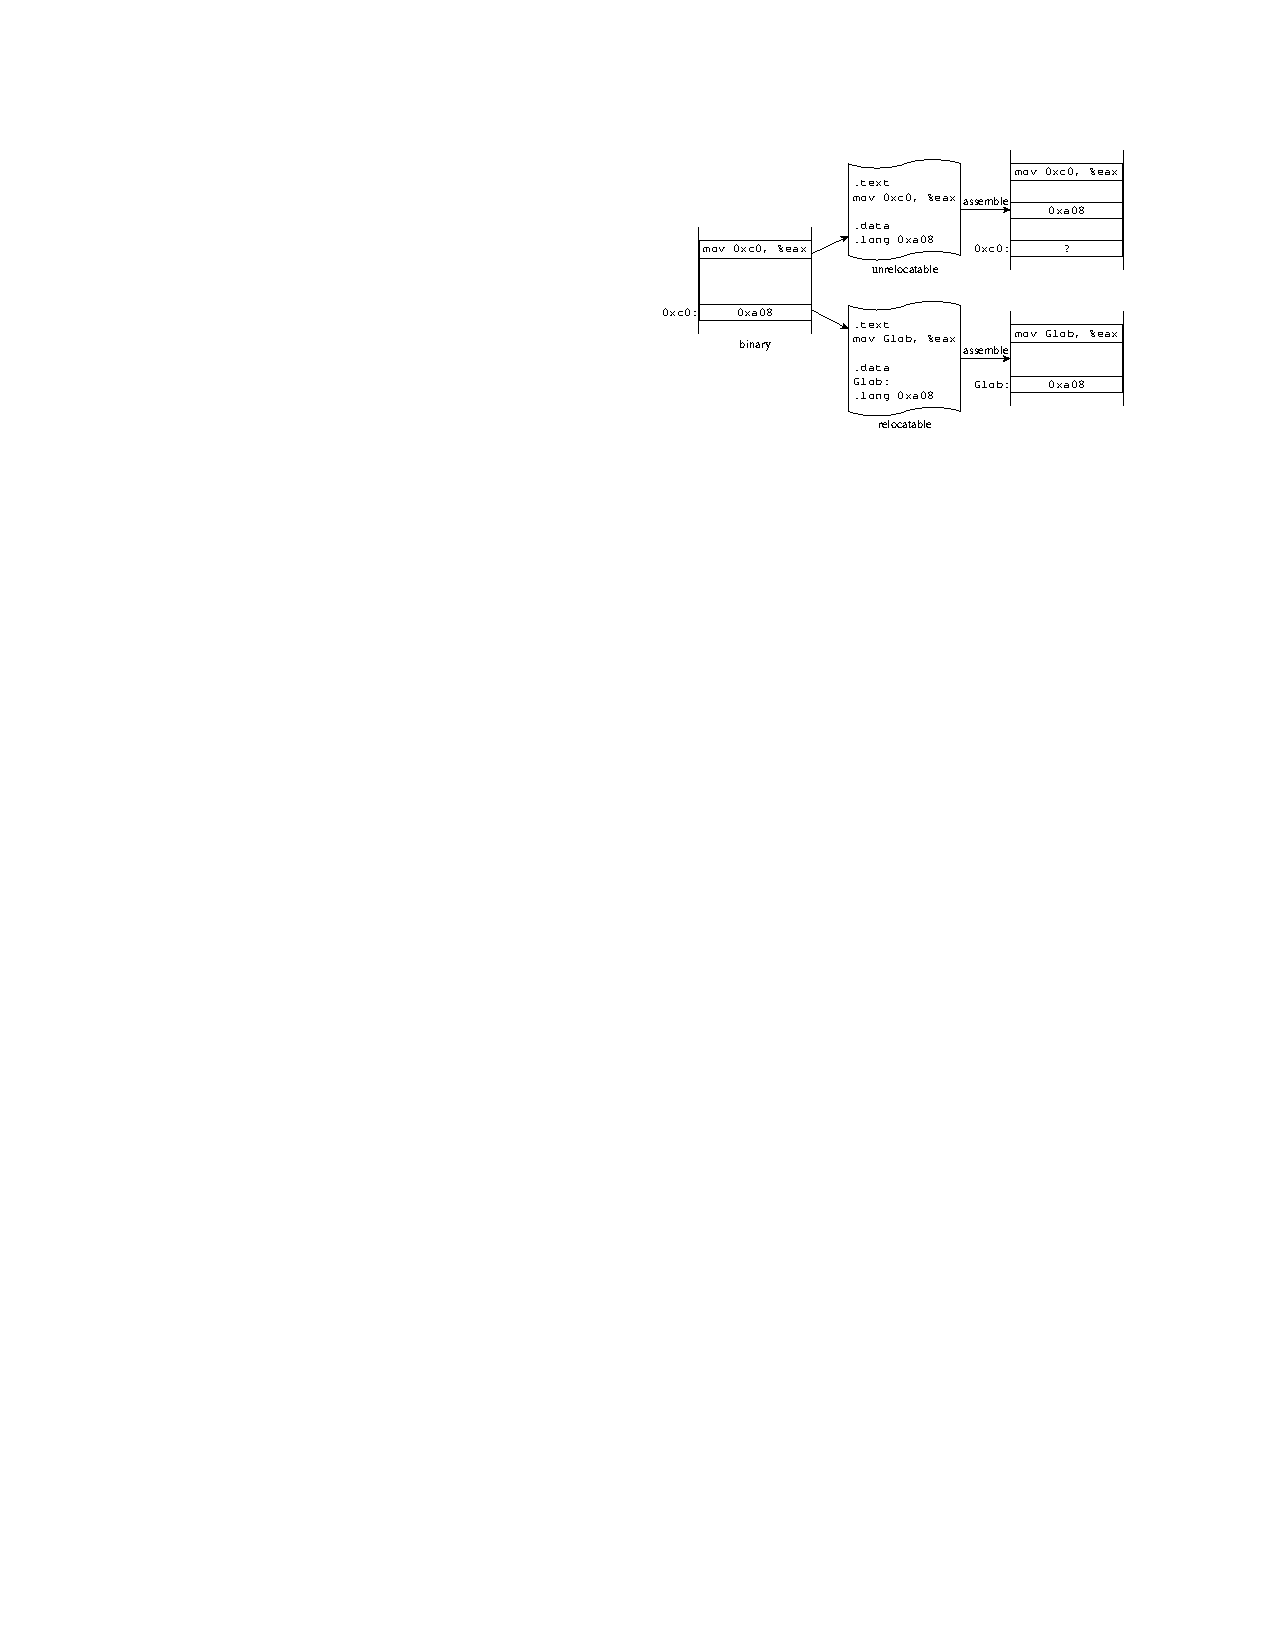
\includegraphics[width=0.8\textwidth]{fig/relocatable.pdf}
  \caption{Relocatable and unrelocatable assembly code~\cite{wang2015reassembleable}.}
  \label{fig:relocatable}
\end{figure}

% \section{Fcuntion Boundary Recovery} \label{sec:challenges-function}

\section{Variables Recovery} \label{sec:challenges-variable}
A variable in source code could be mapped to a low-level register or a memory
offset after compiling to binary.
The variable can be either a local variable, a global variable, or a function
argument.
Classifying a register of memory offset as a variable is known as the variable
recovery problem.
It is challenging to recover variables from stripped binary because information
about variables is lost at compile time.

\begin{figure}[tb]
  \centering
  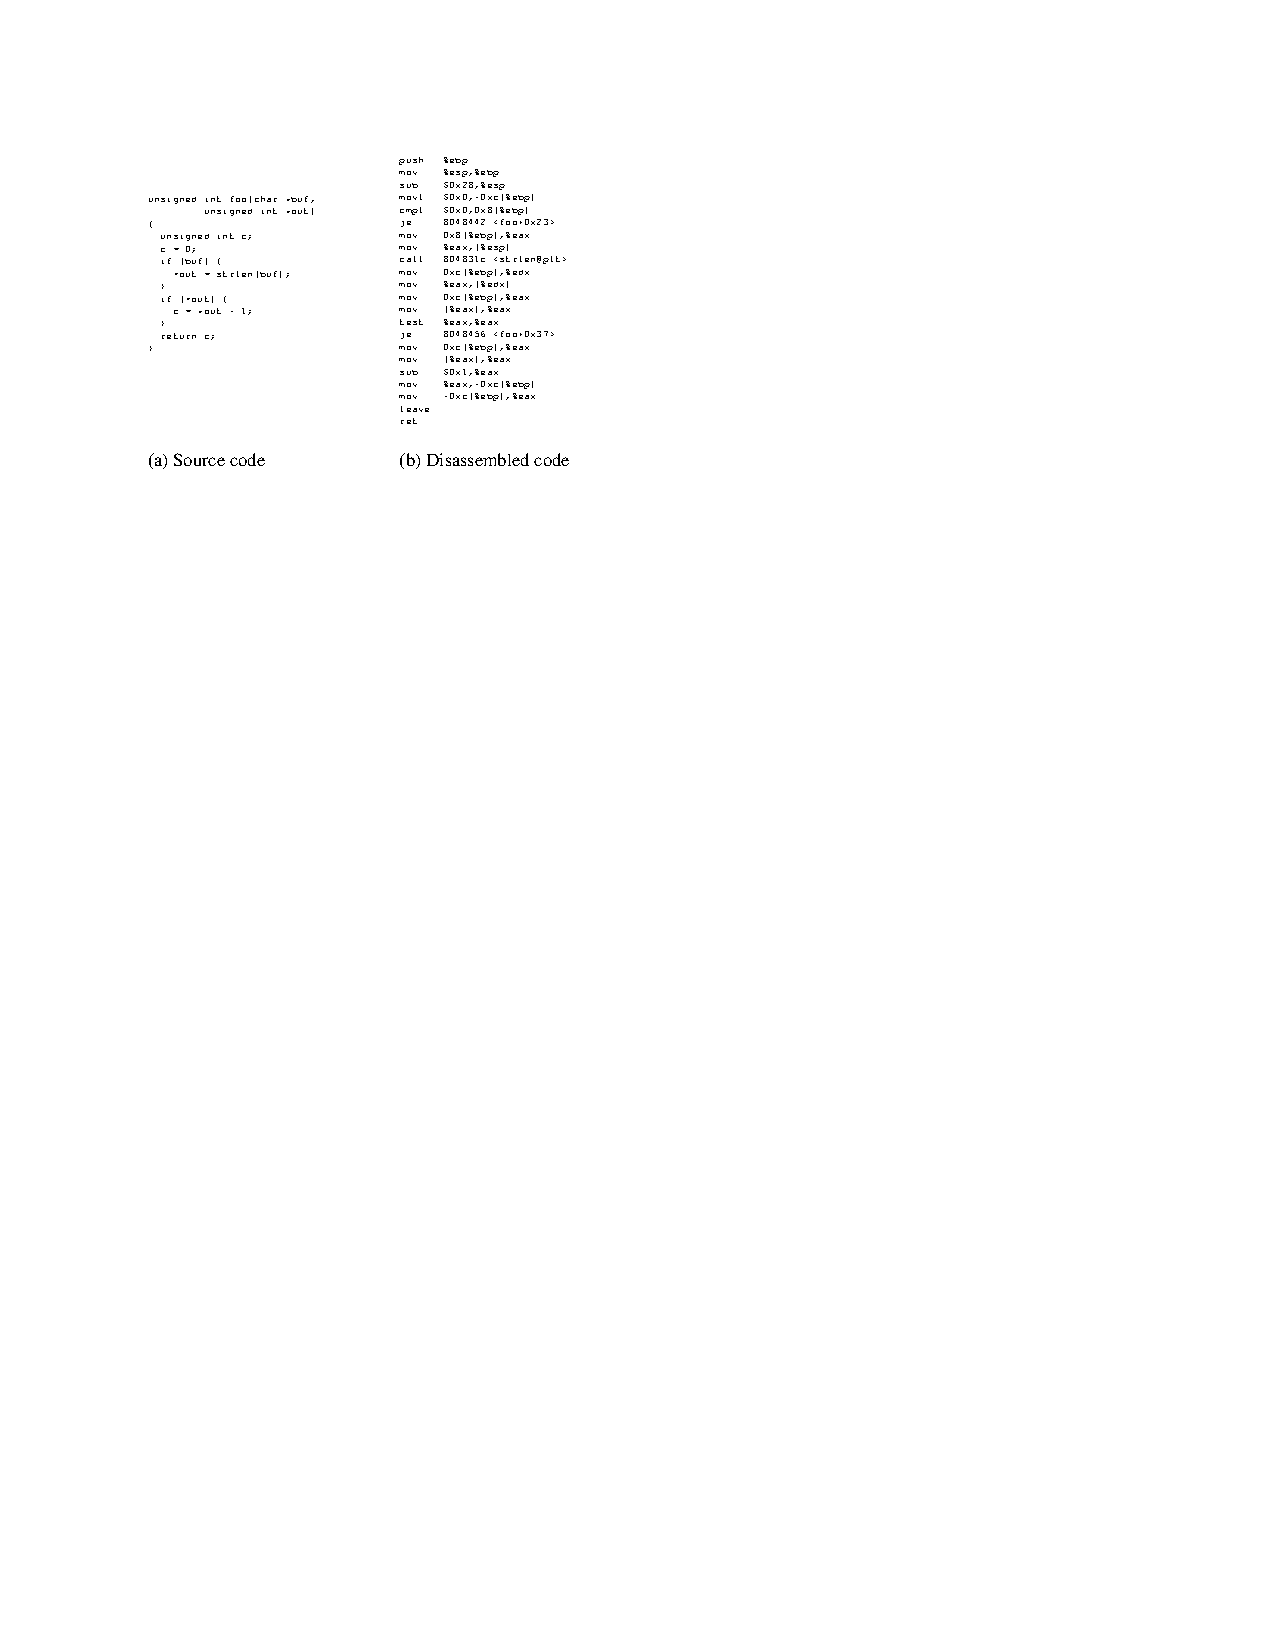
\includegraphics[width=0.6\textwidth]{fig/TIE.pdf}
  \caption{Example of source code and disassembled code~\cite{lee2011tie}.}
  \label{fig:tie}
\end{figure}

For example, consider the disassembled code shown in
\F~\hyperref[fig:tie]{1(b)}, compiled from the source code in
\F~\hyperref[fig:tie]{1(a)}. In the first step, variable recovery should infer
that (at least) two parameters are passed and that the function has one local
variable. Classical approaches recover the variable information by looking at
\textit{access patterns}~\cite{lee2011tie,lin2010automatic}, e.g., one typical
access pattern is accessing a memory block via the ebp register with offsets,
with which we can infer there are two unique parameters (0xc and 0x8).
However, because compiler optimizations may break such patterns, these
approaches are not fully reliable.

\section{Types Recovery} \label{sec:challenges-types}
Similar to the variable recovery problem, to convert the disassembled code to
high-level, \textit{strong typed} IR, we need to recover the types of
variables. We face a similar dilemma as type information is lost at compile
time as well. There are only memory blocks of different sizes at the binary
level, so typical methods seek to infer types from context information.
One straightforward method to infer types is propagating information from
executed \textit{type sinks}, which are calls to functions with known type
signatures, e.g., functions from C standard libraries~\cite{lin2010automatic}.
However, such type sinks are not always available in binary code, some
research formulated constraint-based type inference systems to recover
variable types~\cite{lee2011tie,noonan2016polymorphic}. These methods further
improve accuracy, but are still far from being able to support type-aware
analysis, e.g., pointer analysis.

\section{Control-Flow Structure Recovery} \label{sec:challenges-control-flow}
In the decompilation stage, high-level structured control flow constructs such
as loops, if-then-else, and switch will be recovered from assembly code in the
Control Flow Graph (CFG) form. As discussed in
\S~\ref{subsec:background-decompilation}, modern C decompilers implement a
set of structure templates and are able to guarantee the structure recovery
correctness and also to improve readability
~\cite{brumley2013native,yakdan2015no}. These methods require accurate CFG to
be recovered in advance. However, when indirect jumps exist in the binary
code, recovering CFG needs non-trivial data-flow analysis or dynamic execution
information. Also, indirect jumps may significantly reduce the readability of
decompilation results. In the fact that object-oriented language (such as C++)
compiled binary frequently uses indirect jumps for dynamic dispatch, some
research focuses on reverse engineering of object-oriented
code~\cite{katz2016estimating,schwartz2018using,erinfolami2020devil}.
Nonetheless, due to the complexity of object-oriented code, there is no
standard solution exists. Thus in this survey, we mainly focus on reverse
engineering of C code.


\newpage
